\subsection{Adiabatic speed sensitivity along the conserved EOS trajectory}
\label{sec:adiabatic-sensitivity}
For an adiabatic conversion layer, the temperature-dependent diffusion coefficient must remain inside the rate integral.
We reconstruct the thermodynamic trajectory from upstream conditions, using the slow-front conservation laws and imposing a cold quark interface, \(T(0^+)=0\).
The inputs are \(T(0^-)\) and \(n_B(0^-)\); neither a quark-side chemical potential nor the equilibrated downstream temperature is prescribed.
The upstream phase is QMC-RMF3 pure neutron matter~\cite{Alford:2022bpp,Alford:2023rgp}, with \(n_0=0.16\,\mathrm{fm}^{-3}\), and the bag calibration is \(U_{\rm bag}^{1/4}=189.1566\,\MeV\).
We scan \(1\le n_B(0^-)/n_0\le10\) at \(T(0^-)=0,0.1,5,20,50,100\,\MeV\), refine the boundaries of admissible intervals, and solve for the requested interface compositions within those intervals.
Each slice starts from a 73-point density grid, followed by root refinement and composition-targeted sampling; these reported intervals are numerical scan results rather than a proof excluding arbitrarily narrow disconnected branches.

\paragraph{Conserved trajectory.}
The slow-front constraints are
\begin{equation}
 P(a)=P(0^-),\qquad
 \frac{h(a)}{n_B(a)}=\frac{h(0^-)}{n_B(0^-)}.
 \label{eq:adiabatic-conservation}
\end{equation}
For the massless bag EOS including thermal gluons,
\begin{align}
 P+U_{\rm bag}
 &=\sum_{f=u,d,s}\left(\frac{\mu_f^4}{4\pi^2}+\frac{\mu_f^2T^2}{2}\right)
   +\frac{19\pi^2T^4}{36},\label{eq:adiabatic-pressure}\\
 h&=4(P+U_{\rm bag}),\qquad
 n_B=\frac{4[P(0^-)+U_{\rm bag}]}{h(0^-)/n_B(0^-)}.
 \label{eq:adiabatic-density}
\end{align}
Thus constant baryon density on the quark trajectory follows from conservation and this EOS; it is not an additional frozen-background approximation.
The neutral densities are those of \cref{eq:density}.
The cold interface is found from
\begin{equation}
 P(0^-)+U_{\rm bag}
 =\frac{(\pi^2n_B)^{4/3}}{4\pi^2}
 \left\{1+[1+a(0^+)]^{4/3}+[1-a(0^+)]^{4/3}\right\}.
 \label{eq:adiabatic-cold-interface}
\end{equation}
We retain only \(0<a(0^+)<1\).
For each retained state, solving \cref{eq:density,eq:adiabatic-pressure} at decreasing composition gives \(T(a)\) and all three flavor potentials, ending at \(a(\infty)=0\) and \(\mu_K(\infty)=0\).
The resulting \(T(\infty)\) is an output, and \(\mu_B(a)\) varies along the path.
The neutron-matter roots are required to satisfy the existing physical-branch and residual checks and to agree from at least two seeds.
Supplemental initial seeds recover failed roots without changing these criteria or the production EOS files.

\paragraph{Diffusion-weighted comparison.}
At the same local EOS states for every rate prescription, define
\begin{equation}
 I_{2,\mathrm{model}}=\frac1{n_B}\int_0^{a(0^+)}
 D_K(a)\,\Gamma_{K,\mathrm{model}}(a)\,\dd a,
 \qquad
 \frac{u_{\mathrm{model,est}}(0^-)}{u_{\mathrm{exact,est}}(0^-)}
 =\left(\frac{I_{2,\mathrm{model}}}{I_{2,\mathrm{exact}}}\right)^{1/2}.
 \label{eq:adiabatic-speed-ratio}
\end{equation}
Interface factors and the profile-shape parameter \(\xi\) are identical between models.
We use both terms of the existing diffusion prescription~\cite{Heiselberg:1993cr},
\begin{equation}
 D_K^{-1}=\frac{24\alpha_s^2}{\pi}
 \left[h_D\frac{T^{5/3}}{q_D^{2/3}}+\frac{\pi^3T^2}{12q_D}\right],
 \quad q_D=\sqrt{\frac{6\alpha_s}{\pi}}\frac{\mu_B}{3},
 \quad \alpha_s=0.3,\quad h_D=1.81317,
 \label{eq:adiabatic-diffusion}
\end{equation}
with the local temperature and baryon chemical potential.
The strong coupling enters this transport prescription; the rate still uses the tree-level four-quark channel specified in \cref{sec:conventions}.

\paragraph{The cold endpoint.}
For a fixed interior interface composition, the cold constant-density pressure derivatives give
\begin{equation}
 \left.\frac{\partial P}{\partial a}\right|_{n_B,T=0}
 =\frac{n_B(\mu_d-\mu_s)}3,
 \qquad
 \lim_{T\to0^+}\frac1T\left.\frac{\partial P}{\partial T}\right|_{n_B,a}
 =\frac{\mu_u^2+\mu_d^2+\mu_s^2}{3}.
 \label{eq:adiabatic-cold-derivatives}
\end{equation}
Consequently \(|\dd a/\dd T|\propto T\), whereas \(D_K\propto T^{-5/3}\), so \(D_K\Gamma_K|\dd a/\dd T|\propto T^{-2/3}\) is integrable.
The dimensionless integration coordinate \(z=[T/T(\infty)]^{1/3}\) removes this singularity and runs from the cold interface to equilibrium.
Its EOS Jacobian is obtained by implicit differentiation of \cref{eq:adiabatic-pressure} at fixed density:
\begin{equation}
 \left|\frac{\dd a}{\dd z}\right|
 =\frac{(\partial P/\partial T)_{n_B,a}}{(\partial P/\partial a)_{n_B,T}}
 \,3T(\infty)z^2.
 \label{eq:adiabatic-jacobian}
\end{equation}
The finite cold value of the transformed integrand is
\begin{equation}
 \lim_{z\to0^+}\frac{D_K\Gamma_K}{n_B}\left|\frac{\dd a}{\dd z}\right|
 =\frac{\pi q_D(0^+)^{2/3}\Gamma_K(0^+)T(\infty)^{1/3}
         \sum_f\mu_f(0^+)^2}
 {8\alpha_s^2h_D n_B^2[\mu_d(0^+)-\mu_s(0^+)]}.
 \label{eq:adiabatic-cold-integrand}
\end{equation}
No temperature floor is inserted.
This improper integral defines a formal speed sensitivity with the stated transport law; its finiteness does not establish the validity of local diffusion arbitrarily close to a zero-temperature interface.

\paragraph{Results and diffusion weighting.}
With \(T(0^+)=0\), the interface composition is an output rather than an input.
Eliminating \(n_B\) between \cref{eq:adiabatic-density,eq:adiabatic-cold-interface} gives
\begin{equation}
 1+[1+a(0^+)]^{4/3}+[1-a(0^+)]^{4/3}
 =\left[\frac{(h/n_B)^4}{4\pi^2(P+U_{\rm bag})}\right]^{1/3}_{0^-},
 \label{eq:adiabatic-composition-map}
\end{equation}
so each upstream state \((n_B(0^-),T(0^-))\) fixes one composition, with \(a(0^+)=0\) and \(a(0^+)=1\) at right-hand values \(3\) and \(1+2^{4/3}\).
At fixed \(a(0^+)\), this massless cold-interface problem has a useful scaling property.
All temperatures and chemical potentials scale as \(n_B^{1/3}\), the weak rate as \(n_B^{8/3}\), diffusion as \(n_B^{-1/3}\), and hence \(I_2\) as \(n_B^{4/3}\).
The two-term diffusion law preserves this scaling at fixed \(\alpha_s\).
Therefore the ratios in \cref{eq:adiabatic-speed-ratio} depend on the upstream state only through \(a(0^+)\), and lines of constant ratio in the upstream plane are lines of constant \(a(0^+)\).
Figure~\ref{fig:adiabatic-speed} shows these lines in the \((n_B(0^-),T(0^-))\) plane used for the front-speed contours.
The right side of \cref{eq:adiabatic-composition-map} is evaluated with the same QMC-RMF3 validator on a uniform grid of 49 temperatures from \(0\) to \(120\,\MeV\) and 101 densities from \(n_0\) to \(6n_0\), with no EOS failures.
The grid encloses both boundaries; the \(a(0^+)=1\) boundary reaches \(n_B(0^-)=n_0\) at \(T(0^-)=112.28\,\MeV\).
Each contour level is converted to a composition with the composition-resolved quadrature of this section, whose ratio curves appear in the left panel of Figure~\ref{fig:adiabatic-diffusion}.
At the 128 precisely solved upstream states inside this grid, the linearly interpolated composition differs from the solved one by at most \(2.6\times10^{-3}\).
Only interior compositions are integrated; the largest composition in the quadrature is \(0.995\), and neither endpoint is asserted to be a finite-speed solution.
For \(T(0^-)\leq50\,\MeV\), the scanned densities span the full interior composition interval.
At \(T(0^-)=100\,\MeV\), the density interval is \([1,3.380011)\,n_0\) and the attainable composition interval is \([0.879368,1)\).
Here the composition initially decreases with density, reaches its minimum at \(n_B(0^-)/n_0=1.444184\), and then increases.
Both density roots are saved for the sampled compositions \(0.88,0.885,0.89\); they produce the same speed ratio by the scaling above.
The complete selection contains 153 upstream states at 45 distinct interface compositions, with no unresolved EOS queries.
\par
\begin{table}[tbp]
\centering
\caption{Adiabatic cold-interface benchmarks on the conserved EOS trajectory.
The last two columns give percentage changes of the speed estimate relative to the exact phase-space reference.}
\label{tab:adiabatic-speed}
\begin{tabular}{rrrrrr}
\toprule
\(T(0^-)\) & \(a(0^+)\) & \(n_B(0^-)/n_0\) & \(T(\infty)\) & Eq.~(23) & \(T^0+T^2\)\\
{[MeV]} & & & {[MeV]} & {[\%]} & {[\%]}\\
\midrule
0 & 0.146 & 3.04060 & 8.726 & +3.70 & +0.35 \\
0 & 0.5 & 3.48993 & 31.097 & +16.66 & +0.81 \\
0 & 0.9 & 4.75287 & 63.297 & +56.11 & +0.46 \\
0.1 & 0.146 & 3.04060 & 8.726 & +3.70 & +0.35 \\
0.1 & 0.5 & 3.48993 & 31.097 & +16.66 & +0.81 \\
0.1 & 0.9 & 4.75287 & 63.297 & +56.11 & +0.46 \\
5 & 0.146 & 3.03437 & 8.723 & +3.70 & +0.35 \\
5 & 0.5 & 3.48461 & 31.086 & +16.66 & +0.81 \\
5 & 0.9 & 4.74894 & 63.280 & +56.11 & +0.46 \\
20 & 0.146 & 2.93742 & 8.671 & +3.70 & +0.35 \\
20 & 0.5 & 3.40278 & 30.911 & +16.66 & +0.81 \\
20 & 0.9 & 4.68940 & 63.009 & +56.11 & +0.46 \\
50 & 0.146 & 2.22564 & 8.352 & +3.70 & +0.35 \\
50 & 0.5 & 2.85750 & 29.844 & +16.66 & +0.81 \\
50 & 0.9 & 4.33343 & 61.411 & +56.11 & +0.46 \\
100 & 0.146 & \multicolumn{4}{c}{unavailable in density search range}\\
100 & 0.5 & \multicolumn{4}{c}{unavailable in density search range}\\
100 & 0.9 & 2.08661 & 52.968 & +56.11 & +0.46 \\
\bottomrule
\end{tabular}
\end{table}
The unavailable benchmark compositions at \(T(0^-)=100\,\mathrm{MeV}\) are \(0.146\), \(0.5\).
\begin{table}[tbp]
\centering
\caption{Admissible upstream density intervals in the search range \(1\le n_B(0^-)/n_0\le10\).
Boundary compositions \(0\) and \(1\) are limiting states, excluded from the rate-integral calculation.}
\label{tab:adiabatic-intervals}
\begin{tabular}{rccc}
\toprule
\(T(0^-)\) [MeV] & \(n_B(0^-)/n_0\) interval & limiting \(a(0^+)\) range & status\\
\midrule
0 & (3.000000, 5.297929) & (0.0000, 1.0000) & admissible \\
0.1 & (2.999998, 5.297932) & (0.0000, 1.0000) & admissible \\
5 & (2.993658, 5.294344) & (0.0000, 1.0000) & admissible \\
20 & (2.894983, 5.240216) & (0.0000, 1.0000) & admissible \\
50 & (2.160893, 4.923040) & (0.0000, 1.0000) & admissible \\
100 & [1.000000, 3.380011) & [0.8794, 1.0000) & admissible \\
\bottomrule
\end{tabular}
\end{table}
At \(a(0^+)=0.146,0.5,0.9\), Eq.~(23) gives speed-estimate changes of \(+3.70\%\), \(+16.66\%\), \(+56.11\%\), respectively.
At the same compositions the derived \(T^0+T^2\) prescription changes the estimate by \(+0.35\%\), \(+0.81\%\), \(+0.46\%\).
For \(a(0^+)=0.9\), replacing local diffusion by a common constant on the same thermodynamic trajectory changes the Eq.~(23) ratio from \(1.56107\) to \(1.32678\).


Figure~\ref{fig:adiabatic-diagnostics} shows the temperature, diffusion coefficient, local rate error, and cumulative contribution for a representative trajectory, including the \((\mu_B/3)^5\) variant of Eq.~(23).
On this trajectory the variant gives a speed ratio of \(1.252\), compared with \(1.561\) for Eq.~(23).
The large diffusion coefficient gives additional weight to the cold, unequilibrated part of the path, where the mismatch between the exact cold phase space and Eq.~(23) is substantial.
Figure~\ref{fig:adiabatic-diffusion} repeats the comparison after replacing diffusion by one common constant on each of the same trajectories.
This diagnostic isolates diffusion weighting while keeping the thermodynamic path and all local rates unchanged.
Agreement of the integrated \(T^0+T^2\) prescription with the exact reference is an observed weighted result, not a claim of uniform accuracy of the temperature expansion near equilibrium or at high temperature.
\paragraph{Verification.}
Across 11,016 saved dimensional trajectory samples, the maximum relative pressure and enthalpy-per-baryon residuals are \(6.58\times10^{-13}\), while the neutrality and baryon-density residuals are below \(4\times10^{-15}\).
Every reconstructed trajectory has \(T(0^+)=0\) and \(\mu_K(\infty)=0\); the maximum mismatch between target and solved interface composition is \(8.98\times10^{-12}\).
% Generated by adiabatic_verify.py; do not edit by hand.
Numerical verification covers 45 distinct interface compositions and 143 quadrature records.
Outer-order refinement covers every composition; phase-order and tail checks cover four representative compositions.
The cold-state sweep evaluates 3025 states, with 0 failures and maximum relative pressure and density residuals \(6.66\times10^{-16}\) and \(6.66\times10^{-16}\), respectively.
An independently implemented 40-digit EOS and composition-coordinate integral check the temperature-coordinate Jacobian; the rate and diffusion routines are shared.
\par
\begin{table}[htbp]
\centering
\small
\begin{tabular}{lrr}
\hline
Check & Integral change & Speed-ratio change \\
\hline
Independent coordinate & \(4.19\times10^{-6}\) & \(2.10\times10^{-6}\) \\
EOS iterations 64 to 100 & \(0\) & \(0\) \\
Outer order 12 to 18 & \(9.44\times10^{-6}\) & \(4.72\times10^{-6}\) \\
Phase order 16 to 28 & \(2.22\times10^{-16}\) & \(2.22\times10^{-16}\) \\
Tail 48 to 64 & \(4.44\times10^{-16}\) & \(2.22\times10^{-16}\) \\
Cutoff \(1.00\times10^{-3}\), uncorrected & \(1.30\times10^{-1}\) & \(9.12\times10^{-3}\) \\
Cutoff \(1.00\times10^{-3}\), cold tail added & \(5.39\times10^{-3}\) & \(3.33\times10^{-4}\) \\
Cutoff \(1.00\times10^{-5}\), uncorrected & \(2.88\times10^{-2}\) & \(1.84\times10^{-3}\) \\
Cutoff \(1.00\times10^{-5}\), cold tail added & \(2.61\times10^{-4}\) & \(1.62\times10^{-5}\) \\
Cutoff \(1.00\times10^{-7}\), uncorrected & \(6.26\times10^{-3}\) & \(3.90\times10^{-4}\) \\
Cutoff \(1.00\times10^{-7}\), cold tail added & \(1.22\times10^{-5}\) & \(6.07\times10^{-6}\) \\
\hline
\end{tabular}
\caption{Observed relative numerical changes for the cold-interface adiabatic sensitivity calculation, taking the maximum absolute value over the tested compositions and rate models.
Cutoffs are specified by \(T_{\rm cut}/T(\infty)\); uncorrected rows intentionally omit the cold contribution and are not acceptance checks.
Every independent, refined, and corrected speed ratio agrees within the required relative tolerance \(10^{-3}\).}
\label{tab:adiabatic-verification}
\end{table}
\par

\par
These are semi-analytical sensitivities of a shared-trajectory, fixed-profile speed estimate.
No spatial boundary-value problem, absolute velocity, or rate-dependent change of \(\xi\) has been calculated.

\begin{figure}[p]
 \centering
 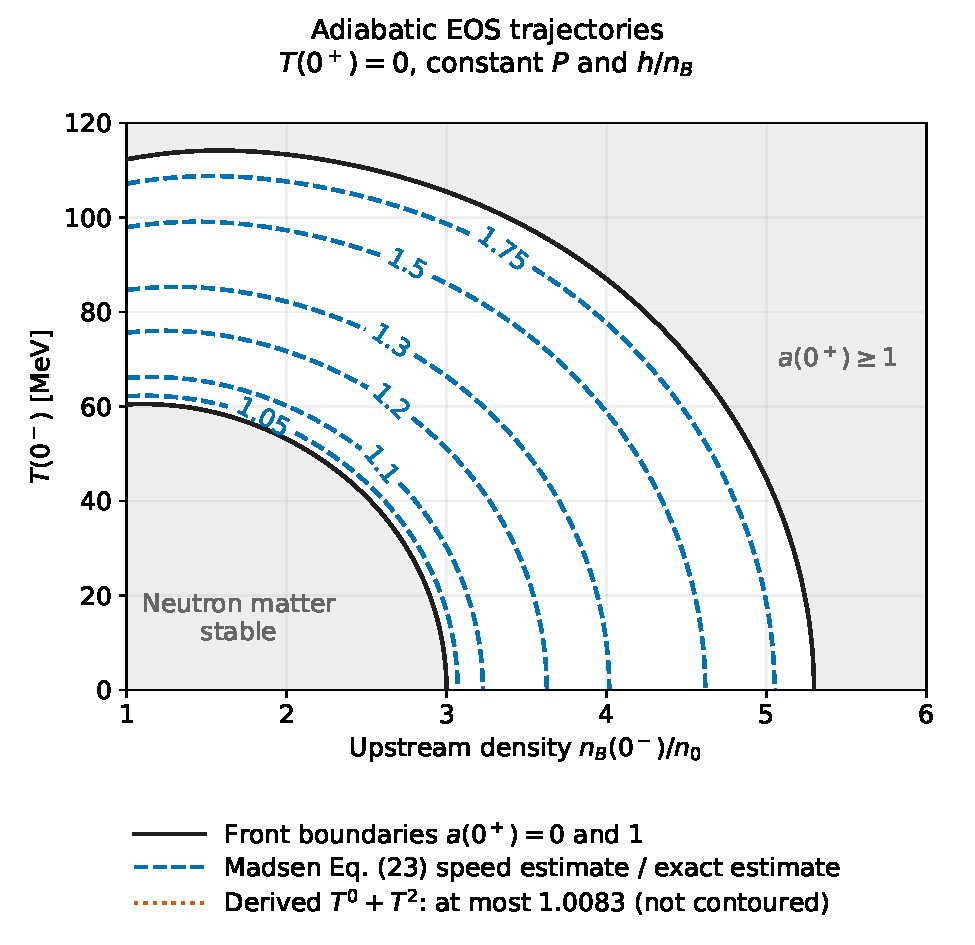
\includegraphics[width=\textwidth]{results/adiabatic-speed-map.pdf}
 \caption{Adiabatic rate-integral speed estimates over upstream QMC-RMF3 neutron-matter states, with \(T(0^+)=0\) and the conserved EOS trajectory.
 Blue dashed contours give the Eq.~(23) estimate divided by the exact phase-space estimate, with local diffusion inside \(I_2\); by massless scaling each contour is a line of constant \(a(0^+)\).
 Black lines are the boundaries \(a(0^+)=0\) and \(a(0^+)=1\); the shaded regions have no cold-interface front.
 The derived \(T^0+T^2\) ratio is at most \(1.0083\) at every computed composition and is not contoured.
 Contours are interpolated from the upstream grid described in the text, whose density range starts at \(n_0\).}
 \label{fig:adiabatic-speed}
\end{figure}
\begin{figure}[p]
 \centering
 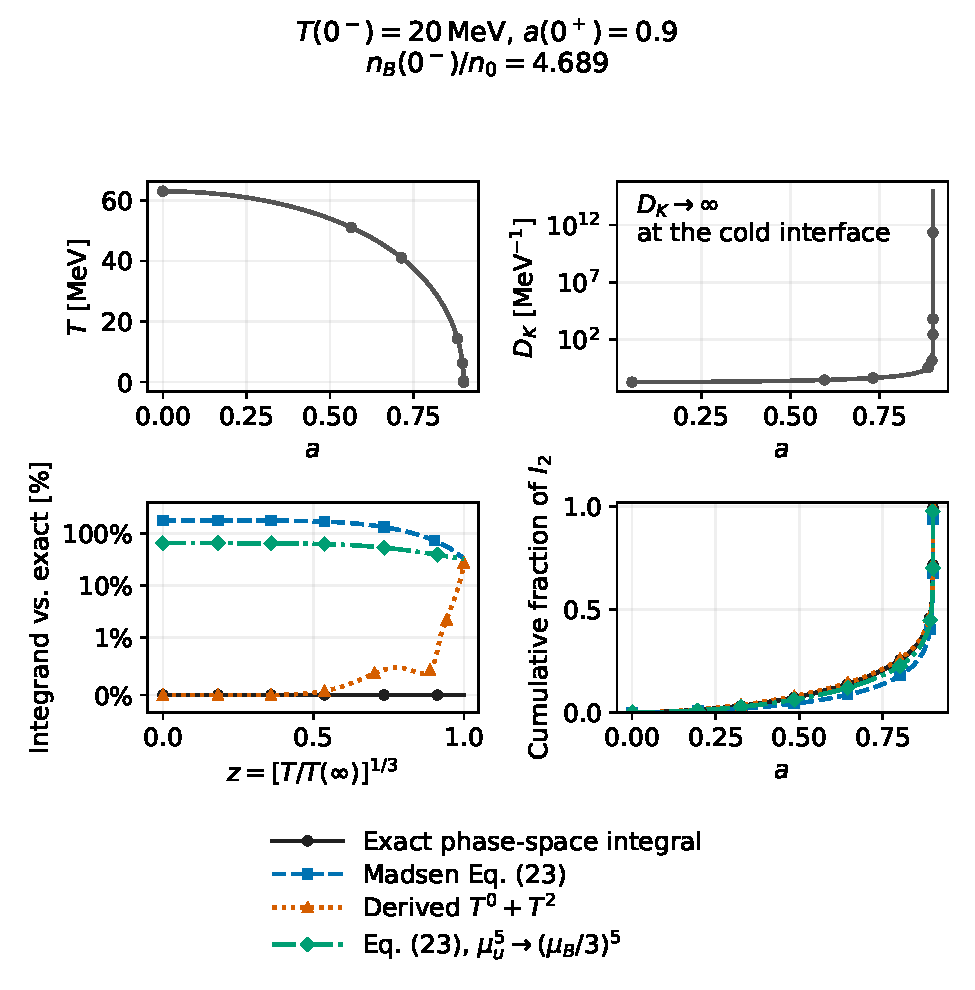
\includegraphics[width=\textwidth]{results/adiabatic-trajectory-diagnostics.pdf}
 \caption{A representative conserved trajectory at \(T(0^-)=20\,\MeV\) and \(a(0^+)=0.9\).
 The upper panels show temperature and local diffusion; diffusion diverges at the cold interface.
 The lower left panel shows each weighted integrand \((D_K\Gamma_K/n_B)|\dd a/\dd z|\) relative to the exact one, in percent on a linear scale within \(1\%\) of zero and logarithmic outside it.
 Because \(D_K\) and the Jacobian are common to all models, this is the local rate error along the path; it is finite at the cold limit \(z=0\).
 Green is Eq.~(23) with \(\mu_u^5\to(\mu_B/3)^5\).
 The lower right panel shows the contribution accumulated from equilibrium to the indicated composition, normalized separately by each model's total \(I_2\).
 Curves connect quadrature samples.}
 \label{fig:adiabatic-diagnostics}
\end{figure}
\begin{figure}[p]
 \centering
 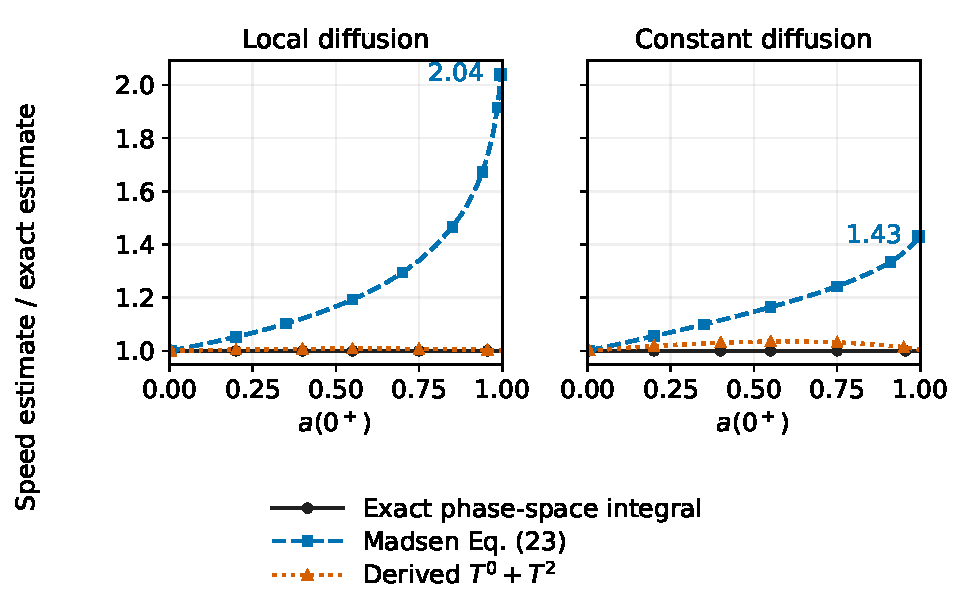
\includegraphics[width=\textwidth]{results/adiabatic-diffusion-weighting.pdf}
 \caption{Local-diffusion and constant-diffusion comparisons on identical adiabatic EOS trajectories.
 In the right panel, a common constant diffusion coefficient cancels from the ratio.
 Both panels retain the temperature rise and varying flavor chemical potentials.
 All three rate prescriptions follow the same color and line conventions as Figure~\ref{fig:speed-sensitivity}.}
 \label{fig:adiabatic-diffusion}
\end{figure}
